\chapter{Evaluation and Analysis of Results}
\label{sec:evaluation}

This chapter presents the evaluation and results of the entity-based sentiment classifier developed in this master's thesis. The chapter is divided in three sections. First one, describes the process of collecting the datasets used to train the classifier and evaluate the proposed solution. The second section is about quality evaluation,  here the overall success of the implemented sentiment classifier is tested and analyzed. Finally, the performance of the classifier is measured and compared with other similar solutions. 

\section{Data Collection and Processing}
\label{sec:collection}

Sentiment classifiers that make use of machine learning methods require a corpus of labeled documents as training data in order to function. Usually the data is manually labeled by evaluators. However, the level of sentiment classification will determine which type of training data is necessary. For sentiment analysis of tweets, these are the most used types of datasets:

\begin{itemize} 
\itemsep0em  

\item \textbf{Document-level}: Documents are labeled based on the sentiment orientation expressed in the whole tweet span without considering the presence of entities or differentiation between expressions. This is the most common type of Twitter sentiment corpus, but it is not useful for an entity based sentiment classifier.

\item \textbf{Entity-level}: Unlike document-level training data, entity-based labeled corpus must reflect the sentiment expressed towards a given entity or query. \autoref{tab:twitter_corpus} shows how the dataset is organized.

\end{itemize}

\begin{table}[H]
\centering
\caption{Entity-based Twitter corpus example.}
\label{tab:twitter_corpus}
\begin{tabular}{|l|c|c|}
\hline
\multicolumn{1}{|c|}{\textbf{Sentiment}} & \textbf{Query/Target} & \textbf{Tweet}                                                                                                                            \\ \hline
Positive                                 & apple                 & \begin{tabular}[c]{@{}c@{}}I'm lovin the iPhone update especially the slide \\ down bar at top of screen =) good job @Apple.\end{tabular} \\ \hline
Negative                                 & twitter               & \begin{tabular}[c]{@{}c@{}}\#Twitter are you freaking kidding me \\ \#wth... http://t.co/zKn2bu5R\end{tabular}                            \\ \hline
Neutral                                  & microsoft             & \begin{tabular}[c]{@{}c@{}}Developers: Let Microsoft Market Your App \\ for Windows Phone http://t.co/QZUqhCxx\end{tabular}               \\ \hline
\end{tabular}
\end{table}

For the development and evaluation of presented entity-based sentiment classifier, a collection of several entity-based labeled corpus was created. This collection is composed by the following datasets:

\begin{itemize} 
\itemsep0em  

\item \textbf{Sanders Analytics\footnote{\url{http://www.sananalytics.com/lab/twitter-sentiment/
}}}:  this dataset is for training and testing sentiment analysis algorithms. It is composed by 5513 manually classified tweets. A 3-class classification method was used (positive, negative, neutral) and each tweet expresses sentiment towards a specific entity.  

\item \textbf{STS-Gold\footnote{\url{http://tweenator.com/index.php?page_id=13
}}}~\cite{saif2013evaluation}: Developed by Mohammad Saif, is a dataset where tweets and targets (entities) are annotated individually. Therefore, only the opinions expressed towards those entities is relevant for result labels.

\item \textbf{SemEval 2015 / 2016}~\cite{rosenthal2015semeval}: SemEval (Semantic Evaluation) is an event held every year where new semantic analysis systems are evaluated. Teams from universities and institutions around the globe submit their solutions to a set of problem tasks defined by the competition committee. One of these task is about Twitter sentiment analysis, therefore, SemEval provides labeled datasets that allow participants to train and evaluate their sentiment classifiers.


\end{itemize}

A normalization process was necessary to remove repeated tweets and noisy tokens from the collection, additionally, a balance between the three different sentiment classes (positive, negative, and neutral) had to be achieve in order to guarantee effective performance of the support vector machine. As a result, \autoref{tab:datasets_summary} shows a summary of the collected tweets. 70\% of the 4900 labeled tweets is used as training data leaving a 30\% for evaluation and testing porpoises. 

\begin{table}[H]
\centering
\caption{Datasets Summary}
\label{tab:datasets_summary}
\begin{tabular}{|l|c|c|c|c|}
\hline
\multicolumn{1}{|c|}{{\color[HTML]{000000} \textbf{Dataset}}} & {\color[HTML]{000000} \textbf{No. of Tweets}} & \textbf{\#Negative} & \textbf{\#Neutral} & \textbf{\#Positive} \\ \hline
{\color[HTML]{000000} Sanders Analytics}                      & {\color[HTML]{000000} 5513}                   & 654                 & 2503               & 570                 \\ \hline
STS-Gold                                                      & 498                                           & 177                 & 139                & 192                 \\ \hline
SemEval 2016                                                  & 2825                                          & 862                 & 965                & 998                 \\ \hline
SemEval 2015                                                  & 1105                                          & 213                 & 422                & 470                 \\ \hline
Normalization                                                 & 4900                                          & 1634                & 1633               & 1633                \\ \hline
\end{tabular}
\end{table}


\section{Quality Evaluation}
In order to measure the quality of the entity-based sentiment classifier developed in this master's thesis, standard evaluation metrics were considered. Therefore, both correct and incorrect predictions must be measured to calculate aforementioned metrics. \autoref{tab:confusion_matrix} presents a three-class confusion matrix which is used to visualize the level of accuracy of predicted data against test datasets.   


\begin{table}[H]
\centering
\caption{3-Class Confusion Matrix}
\label{tab:confusion_matrix}
\begin{tabular}{|l|c|c|c|}
\hline
\multicolumn{1}{|c|}{{\color[HTML]{000000} \textbf{Data Class}}} & {\color[HTML]{000000} \textbf{Classified as Pos}} & \textbf{Classified as Neg} & \textbf{Classified as Neu} \\ \hline
{\color[HTML]{000000} \textbf{Positive}}                         & {\color[HTML]{036400} true positive}              & false negative             & false neutral              \\ \hline
\textbf{Negative}                                                & false positive                                    & {\color[HTML]{036400} true negative}              & false neutral              \\ \hline
\textbf{Neutral}                                                 & false positive                                    & false negative             & {\color[HTML]{036400} true neutral}               \\ \hline
\end{tabular}
\end{table}

Using the confusion matrix illustrated in \autoref{tab:confusion_matrix}, several different metrics were calculated for the evaluation of the classifier. The scoring metrics considered in this project are the following:

\begin{itemize} 
\itemsep0em  

\item \textbf{Precision}: Precision is the rate of correct predictions over the universe of predictions (true + false). For the positive class, precision is defined as follows:
    
    \begin{equation}
        precision = \frac{\text{true positive}}{\text{true positive} + \text{false positive}} 
    \end{equation}
    
\item \textbf{Recall}: is the fraction of relevant tweets that are successfully predicted.  Continuing with positive class example, recall is defined as:

    \begin{equation}
        recall = \frac{\text{true positive}}{\text{true positive} + \text{false negative} + \text{false neutral}} 
    \end{equation}
    
\item \textbf{Accuracy}: is an overall representation of correct predictions. For a three-class classifier, it is defined as follows:

    \begin{equation}
        accuracy = \frac{\text{total correct prediction}}{\text{total correct prediction} + \text{total incorrect prediction}} 
    \end{equation}

\item \textbf{F-Score}: (F-Measure) is defined as the combination of precision and recall. This is the result formula for class \textit{positive}:

    \begin{equation}
        Fscore = 2 * \frac{precision_{positive} * recall_{positive}}{precision_{positive} + recall_{positive}} 
    \end{equation}

\end{itemize}

Based on 4900 collected tweets (datasets) and previews described metrics, a 4-fold cross validation test was performed in proposed entity-based sentiment classifier. The results are presented in \autoref{tab:first_results}. According to obtained results, proposed classifier achieved an accuracy of 0.635 (64\%).
\begin{table}[H]
\centering
\caption{Precision, Recall and F-Score results}
\label{tab:first_results}
\begin{tabular}{l|c|c|c}
\hline
\multicolumn{1}{|c|}{{\color[HTML]{000000} \textbf{Data Class}}} & {\color[HTML]{000000} \textbf{Precision}} & \textbf{Recall} & \multicolumn{1}{c|}{\textbf{Fscore}} \\ \hline
\multicolumn{1}{|l|}{{\color[HTML]{000000} Positive}}            & {\color[HTML]{000000} 0.594}              & 0.668           & \multicolumn{1}{c|}{0.629}           \\ \hline
\multicolumn{1}{|l|}{Negative}                                   & 0.650                                     & 0.615           & \multicolumn{1}{c|}{0.632}           \\ \hline
\multicolumn{1}{|l|}{Neutral}                                    & 0.669                                     & 0.622           & \multicolumn{1}{c|}{0.645}           \\ \hline
Total:                                                           & 0.637                                     & 0.635           & 0.635                               
\end{tabular}
\end{table}

Results in \autoref{tab:first_results} show that the class \textit{positive} achieved the lowest performance while \textit{neutral} class obtained the highest. \textit{Neutral} class tends to get better results since its classification depends on the absence of sentiment expressions. Therefore, polarity classification represents a bigger challenge because of possible presence of negation context and sarcasm comments.

\subsection{Features Contribution}

As explained in \autoref{sec:feature_generation}, the generation of feature vectors is an essential process for sentiment classifiers. Hence, the contributions made by each of the features generated for proposed classifier are illustrated in \autoref{tab:contributions} and \autoref{fig17:contributions_graph}. 

\begin{table}[H]
\centering
\caption{Features contribution details}
\label{tab:contributions}
\begin{tabular}{l|l|l|l|l}
\multicolumn{1}{c|}{{\color[HTML]{000000} \textbf{}}} & \textbf{F-Score} & \textbf{Accuracy} & \textbf{Diff-F} & \textbf{Diff-A} \\ \hline
{\color[HTML]{000000} \textbf{All Features}}          & 0.629            & 0.635             &                 &                 \\ \hline
/ - Unigrams                                          & 0.619            & 0.626             & - 0,01          & - 0,009         \\ \hline
/ - Emoticons                                         & 0.618            & 0.626             & - 0,01          & - 0,009         \\ \hline
/ - Content                                           & 0.536            & 0.571             & - 0,093         & - 0,064         \\ \hline
/ - POS Tags                                          & 0.541            & 0.576             & - 0,088         & - 0,059         \\ \hline
/ - Lexicon                                           & 0.362            & 0.495             & - 0,267         & - 0,14          \\ \hline
\end{tabular}
\end{table}

\begin{figure}[H]
    \centering
    \caption[Features Contribution Graph]{Feature Contributions Graph}
    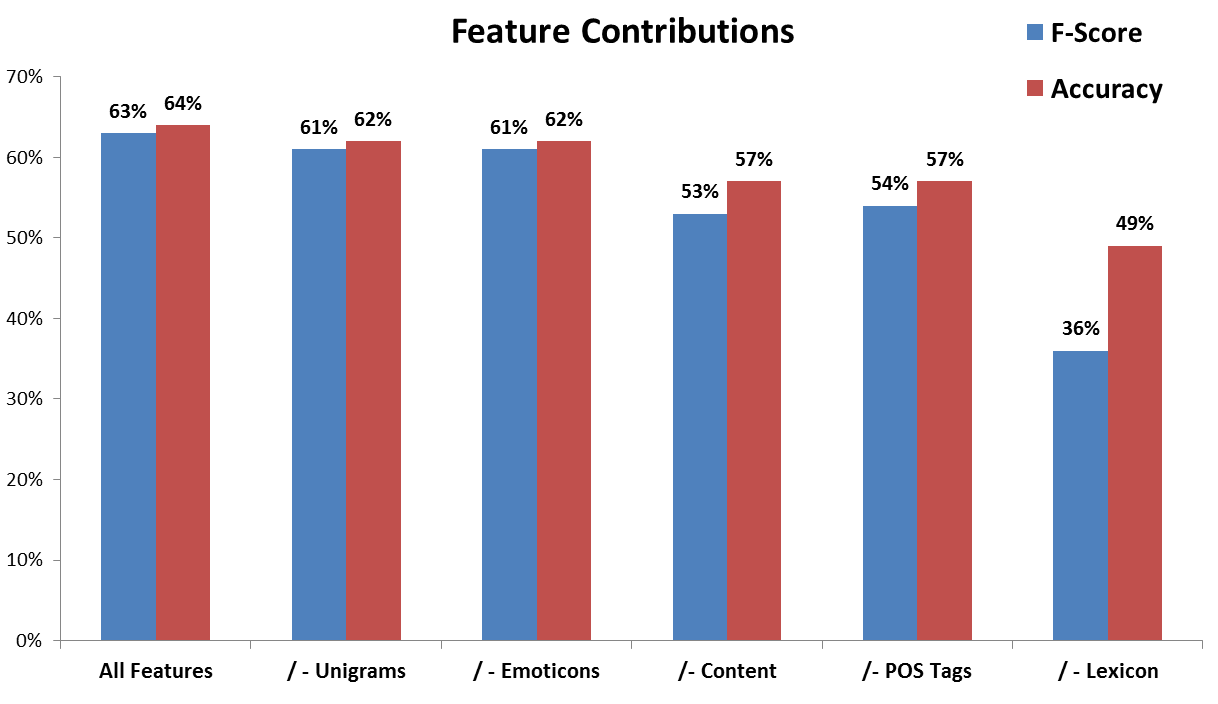
\includegraphics[width=\linewidth]{17_contributions_graph}
    \label{fig17:contributions_graph}
\end{figure}

These results show how important the lexicon features are to the overall performance of the classifier, the contribution of the seven state-of-the-art lexical resources is significantly higher than the contributions obtained by other features. Content and POS Tags features achieved very interesting results surpassing unigrams and emoticons features by a considerable margin. Although unigrams and bag-of-words are some of the most popular features, the evaluation results yield insignificant contributions from this vector. Therefore, its possible to assume that in an entity-based classification approach, n-grams might not have the same contribution impact as in document-level sentiment classifiers.   

\subsection{Quality Comparison}

In order to extend the evaluations made to proposed sentiment classifier, a performance comparison between this master's thesis solution and two additional sentiment classification tools was made. The following tools were considered: 

\begin{itemize} 
\itemsep0em  

\item \textbf{Former SentiTrack Classifier}: SentiTrack as described in \autoref{sec:sentitrack} requires a sentiment classifier to project public's opinion about specific companies in Twitter. Proposed sentiment classifier aims to replace the already existing classifier which is referred as \textit{former SentiTrack classifier}. Former classifier uses unsupervised techniques such as lexicons and linguistic rules to classify tweets as positive, negative or neutral. Also, it is based on a very popular NodeJS module called \textit{Sentiment}\footnote{\url{https://www.npmjs.com/package/sentiment}}. 

\item \textbf{CompendiumJS\footnote{\url{https://github.com/Ulflander/compendium-js}}}: is a suit of natural language processing tools for NodeJS platform. This module provides a lexicon-based sentiment classifier capable of perform three-class classification. 

\end{itemize}

\begin{figure}[H]
    \centering
    \caption[Classifiers Comparison Graph]{Classifiers Comparison Graph}
    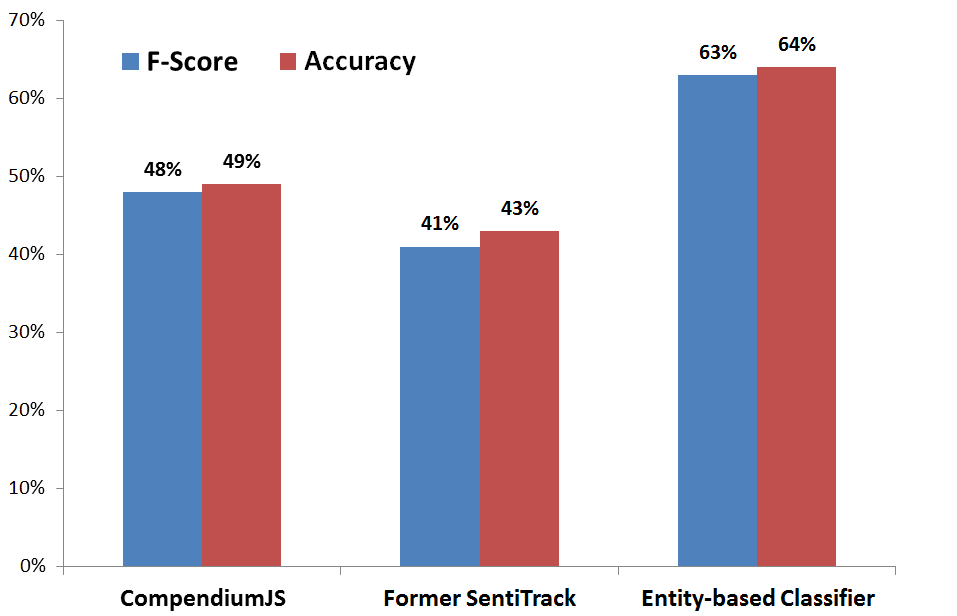
\includegraphics[width=\linewidth]{18_comparison_graph}
    \label{fig18:comparison_graph}
\end{figure}

\autoref{fig18:comparison_graph} illustrates the results obtained by a 4-fold cross validation test of 4900  target-labeled tweets (\autoref{sec:collection}) performed over three sentiment classifiers including the one developed and proposed in this master's thesis. The results show a significant difference in F-Score and Accuracy between the entity-based classifier and the other two tools. Former SentiTrack classifier's poor performance is consequence of its simplicity, it is based on one single lexical resources \textit{AFINN} with no consideration of negation context and emoticons. The difference between results is related to the classification techniques, most state-of-the-art sentiment classifiers for Twitter use supervised methods capable of analyze many tweet-specific features. Hence, presented solution make use of machine learning methods.  


\section{Performance Evaluation}

A performance evaluation measures how long will take proposed classifier to process a given amount of tweets. This is a very important evaluation given that one of the objectives of this research project is to develop a sentiment classifier capable of function under real-time processing systems such as SentiTrack. Additionally, the performance test is also done to former SentiTrack classifier and CompendiumJS in order to compare resulting processing times. These are the evaluation environment specifications: 

\begin{itemize} 
\itemsep0em  

\item \textbf{Processor}: Intel Core i5-2320 CPU @ 3.00GHz

\item \textbf{Memory RAM}: 8 GB 

\item \textbf{Operative System}: 64 bits Windows 7

\end{itemize}

The results are shown in \autoref{tab:performance_results}, they reflect a large difference in performance time between former SentiTrack classifier and proposed solution. Can be inferred, that the complex pipeline of processes required by the entity-based classifiers and the usage of supervised techniques have an impact in classification time. However, the performance achieved by proposed solution is good enough to cope with real-time processing enviroments like SentiTrack.  

\begin{table}[H]
\centering
\caption{Performance test results}
\label{tab:performance_results}
\begin{tabular}{l|c}
\multicolumn{1}{c|}{{\color[HTML]{000000} \textbf{}}} & \textbf{1000 Tweets} \\ \hline
{\color[HTML]{000000} \textbf{Entity-based (ms)}}     & 3447.054             \\ \hline
\textbf{Former SentiTrack (ms)}                       & 323.310              \\ \hline
\textbf{CompendiumJS (ms)}                            & 2357.886             \\ \hline
\end{tabular}
\end{table}

\section{SentiTrack Experiment}

After proposed/built entity-based sentiment classifier was integrated to SentiTrack, an experiment was performed. This experiment intends to find a correlation between the two variables (social media sentiment, stock market prices) filtering and classifying live tweets; as well as stock market movements, over a week for a set of 6 companies. Moreover, a correlation test was done over collected sentiments and stock market data for each evaluated company. 

The overall results were very positive in comparison to previews SentiTrack experiments where the former classifier was used, evidence of a moderate correlation was found on 3 out of 6 companies with a maximum correlation of 0.84 (84\%). These results prove a successful integration between proposed/built sentiment classifier and SentiTrack, which will provide a more accurate analysis for future experiments. 


